\documentclass[11pt,a4paper]{article}

\usepackage[utf8]{inputenc}    % Umlaute in der .tex-Datei
\usepackage[T1]{fontenc}       % Korrekte Silbentrennung
\usepackage{lmodern}           % Bessere Schrift
\usepackage{graphicx}          % Für Logo/Grafiken
\usepackage[left=3.5cm, right=2.0cm, top=2.5cm, bottom=2.5cm]{geometry} % Seitenränder anpassen bei Bedarf
\usepackage{hyperref}
\usepackage{xcolor}
\usepackage{setspace}
\onehalfspacing
\definecolor{htwgreen}{HTML}{76B900}
\usepackage[ngerman, num]{isodate}
\monthyearsepgerman{\,}{\,}
\usepackage[ngerman]{babel}
\usepackage[backend=biber,style=numeric,sorting=none]{biblatex}
\addbibresource{./references.bib}
\usepackage{float}
\usepackage[autostyle=true,german=quotes]{csquotes}
\usepackage{listings}
\usepackage{amsmath}

\definecolor{codegreen}{rgb}{0,0.6,0}
\definecolor{codegray}{rgb}{0.5,0.5,0.5}
\definecolor{codepurple}{rgb}{0.58,0,0.82}
\definecolor{backcolour}{rgb}{0.95,0.95,0.92}

\lstdefinestyle{mystyle}{
    backgroundcolor=\color{backcolour},   
    commentstyle=\color{codegreen},
    keywordstyle=\color{magenta},
    numberstyle=\tiny\color{codegray},
    stringstyle=\color{codepurple},
    basicstyle=\ttfamily\footnotesize,
    breakatwhitespace=false,
    breaklines=true,
    captionpos=b,
    keepspaces=true,
    numbers=left,
    numbersep=5pt,
    showspaces=false,
    showstringspaces=false,
    showtabs=false,
    tabsize=2
}

\lstset{
    style=mystyle,
    language=Python,
    frame=single,
    showstringspaces=false,
    inputencoding=utf8,
    literate={ä}{{\"a}}1 {ö}{{\"o}}1 {ü}{{\"u}}1 {Ä}{{\"A}}1 {Ö}{{\"O}}1 {Ü}{{\"U}}1 {ß}{{\ss}}1,
}

% Für Überschriften etwas schönere Darstellung (optional):
% \usepackage{titlesec}
% \titleformat{\section}{\bfseries\Large}{\thesection}{1em}{}
% \titleformat{\subsection}{\bfseries\normalsize}{\thesubsection}{1em}{}

% \onehalfspacing % 1,5-zeiliger Abstand (ggf. anpassen)

\begin{document}

% Titelseite
\begin{titlepage}
    \centering
    
    
\includegraphics[width=4cm]{./bilder/S04_HTW_Berlin_Logo_pos_FARBIG_RGB.jpg}\\[1.0cm]
    \rule{\linewidth}{0.5pt}\\[0.7cm]
    
    {\color{htwgreen}\bfseries\Large Eignung von Large Language Models (LLMs) zur Generierung von Python Code zur
    Datenanalyse}\\[0.5cm]
    \rule{\linewidth}{0.5pt}\\[2.0cm]
    {\large Bachelorarbeit}\\[1.5cm]
    
    % Name des Studiengangs, Fachbereich, etc.
    {\large Name des Studiengangs}\\
    {\LARGE Wirtschaftsinformatik}\\[0.3cm]
    {\color{htwgreen}\LARGE \textbf{Fachbereich 4}}\\[1.5cm]
    
    {vorgelegt von}\\
    {\LARGE Maurice Krüger}\\[3cm]
    
    % Datum, Ort
    {\Large Datum:}\\
    Berlin, \today\\[2.5cm]

    % Gutachter
    {\LARGE
    \begin{tabular}{l l}
        Erstgutachter:  & Prof. Dr.-Ing. Ingo Claßen \\
        Zweitgutachter: & Prof. Dr. Axel Hochstein \\
    \end{tabular}
    }

\end{titlepage}

\textbf{
    Abstract\\
    Diese Bachelorarbeit untersucht die Eignung moderner Large Language Models (LLMs) für die automatisierte Generierung von Python-Code im Kontext typischer Datenanalyseaufgaben. Dabei wird zunächst ein Überblick über die theoretischen Grundlagen von LLMs und der Programmiersprache Python gegeben. Anschließend werden in einer empirischen Untersuchung Codebeispiele durch den Marktführer ChatGPT mit dem Sprachmodell GPTo1 erzeugt und mit manuell geschriebenen Skripten verglichen. Die Bewertung erfolgt anhand mehrerer Kriterien wie Korrektheit, Performanz sowie Verständlichkeit des generierten Codes. Abschließend werden Empfehlungen für den praktischen Einsatz von LLMs in der Datenanalyse abgeleitet sowie ein Ausblick auf zukünftige Entwicklungen gegeben.
}
\newpage

% Inhaltsverzeichnis

\tableofcontents
\newpage

% Einleitung

\section{Einleitung}
\label{sec:einleitung}
\subsection{Problemstellung und Forschungsfragen}
\label{sec:forschungsfragen}
Die schnelle Entwicklung von Large Language Models (LLMs), wie zum Beispiel ChatGPT, hat in den letzten Jahren sowohl im privaten als auch im beruflichen Bereich viel Aufmerksamkeit erregt. Ursprünglich wurden LLMs hauptsächlich zur Lösung alltäglicher Probleme und der Verarbeitung und Erzeugung menschlicher Sprache eingesetzt, doch zunehmend zeigt sich, dass sie auch Programmiercode in verschiedenen Sprachen erstellen können. Besonders in der Programmiersprache Python – einer weit verbreiteten Sprache für Datenanalyse und Machine Learning – sind die Fortschritte in der automatisierten Code-Generierung durch LLMs bereits bemerkenswert\cite{NEURIPS2023_43e9d647,chen2021evaluatinglargelanguagemodels}.

Aktuelle Forschungsarbeiten konzentrieren sich auf die systematische Bewertung von solch generierten Codes, um Fehlerquellen und Qualitätsmerkmale zu bemessen. Die Bereitstellung öffentlicher Evaluierungsdatensätze und -frameworks, wie etwa \emph{HumanEval}\cite{chen2021evaluatinglargelanguagemodels} oder \emph{EvalPlus}\cite{evalplus}, ermöglicht standardisierte Vergleichsstudien verschiedener LLMs. Dies eröffnet neue Anwendungsfelder im Bereich der Datenanalyse: Anstatt den Code manuell zu schreiben, könnten Nutzer in Zukunft lediglich ihre Anforderungen in natürlicher Sprache formulieren und das Modell würde diese für den Nutzer umsetzen\cite{nijkamp2023codegenopenlargelanguage}.

Vor diesem Hintergrund stellt sich die Frage, ob und inwiefern LLMs tatsächlich qualitativ hochwertigen Python-Code für datenanalytische Aufgaben erzeugen können und wie dieser Code im Vergleich zu manuell geschriebenen Code abschneidet. Auch die möglichen Grenzen dieser automatisierten Generierung, wie etwa in Bezug auf Performanz, Wartbarkeit oder Fehlerraten, sind hierbei von großer Bedeutung\cite{wang2021codet5identifierawareunifiedpretrained}.

Daraus ergibt sich die zentrale \textbf{Hauptforschungsfrage}:

\begin{quote}
    \emph{Inwieweit eignen sich Large Language Models (LLMs) zur Durchführung gängiger Datenanalyseaufgaben in Python, und wie schneidet dieser Code im Vergleich zu manuell geschriebenen Code hinsichtlich Effizienz, Korrektheit und Wartbarkeit ab?}
\end{quote}

Zur weiteren Strukturierung dieser Hauptfrage werden mehrere Unterfragen hinzugezogen:
\begin{itemize}
    \item \textbf{Qualität \& Korrektheit:} Wie qualitativ hochwertig ist dieser generierte Code hinsichtlich Syntax und Implementierung von Analyseaufgaben (z.\,B. Datenfilterung, Modellierung)?
    \item \textbf{Effizienz \& Performanz:} Inwieweit entspricht der automatisch erzeugte Code modernen Standards bezüglich Laufzeit und Ressourcenverbrauch?
    \item \textbf{Wartbarkeit \& Verständlichkeit:} Wie gut lässt sich der generierte Code verstehen, dokumentieren und erweitern?
    \item \textbf{Einsatzgebiete \& Grenzen:} Für welche spezifischen Aufgaben in der Datenanalyse ist der Einsatz von LLMs sinnvoll und wo stoßen diese an ihre Grenzen?
\end{itemize}

\subsection{Relevanz der Thematik}
Die Fähigkeit, Programmiercode mit Hilfe von LLMs zu erstellen, könnte die Entwicklungsprozesse erheblich beschleunigen und neue Nutzergruppen anziehen, die bisher wenig Erfahrung mit Programmierung hatten. Besonders in der Datenanalyse können viele Arbeitsschritte – vor allem wiederkehrende Aufgaben, wie das Erstellen von Standard-Pipelines zur Datenbeschaffung- und bereinigung – automatisiert werden. Gleichzeitig gibt es jedoch Herausforderungen in Bezug auf Performanz, Wartbarkeit und Transparenz.

\subsection{Zielsetzung}
Das Ziel dieser Arbeit ist es, herauszufinden, wie gut moderne LLMs (Large Language Models) für die automatische Code-Generierung in der Datenanalyse mit Python geeignet sind. Dafür wird in einem Experiment Code von einem LLM generiert und mit manuell geschriebenem Code verglichen. Der Vergleich basiert auf Kriterien wie Korrektheit, Performance und Wartbarkeit. Auf Basis der Ergebnisse werden Empfehlungen für den Einsatz von LLMs in der Praxis gegeben und deren Grenzen diskutiert. Zum Schluss wird ein Ausblick darauf gegeben, wie sich diese Technologie in Zukunft weiterentwickeln könnte und welche Auswirkungen das auf Aufgaben in der Datenanalyse haben könnte\cite{chen2021evaluatinglargelanguagemodels,evalplus}.

\subsection{Aufbau der Arbeit}
Nach dieser Einleitung (Kapitel \ref{sec:einleitung}) folgt in Kapitel \ref{sec:grundlagen} eine Darstellung der \textbf{Grundlagen}, dazu gehört eine Einführung in Large Language Models, die Programmiersprache Python und die automatisierte Code-Generierung. Kapitel \ref{sec:llms_programmierung} gibt einen Überblick über den aktuellen Stand der Forschung, in dem verschiedene LLM-Modelle, Publikationen und Evaluationstechniken vorgestellt werden. Darauf aufbauend wird in Kapitel \ref{sec:methodik} die \textbf{Methodik} der Arbeit erläutert. Kapitel \ref{sec:auswertung} enthält dann die \textbf{Auswertung} der gewonnenen Daten sowie den Vergleich von durch ein LLM generierten und manuell geschriebenen Code. Kapitel \ref{sec:fazit} fasst die Ergebnisse zusammen, beantwortet die Forschungsfragen und gibt einen \textbf{Ausblick} auf weitere Entwicklungen. Schließlich enthält Kapitel \ref{sec:anhang} den \textbf{Anhang}, einschließlich Literaturverzeichnis und relevanter Dokumentationen.

% Theorieteil

\section{Grundlagen}
\label{sec:grundlagen}
Im folgenden Kapitel werden die theoretischen und technischen Grundlagen vorgestellt, die für das Verständnis dieser Arbeit notwendig sind. Abschnitt~\ref{sec:LLMs} beschäftigt sich mit den Large Language Models, ihrer Funktionsweise und ihrer Bedeutung in der Code-Generierung. Danach wird in Abschnitt~\ref{sec:Python} das Potenzial der Programmiersprache Python für die Datenanalyse erläutert, bevor Abschnitt~\ref{sec:AutoCode} das Konzept der automatisierten Code-Generierung behandelt.

\subsection{Einführung Large Language Models}
\label{sec:LLMs}
Bei großen Sprachmodellen (LLMs) handelt es sich um KI-Systeme, die mithilfe moderner Deep-Learning-Methoden entwickelt wurden, um natürliche Sprache zu verstehen, selbst Texte zu generieren und mit Kontext zu interpretieren\cite{naveed2024comprehensiveoverviewlargelanguage}. Diese Modelle basieren auf Transformer-Architekturen, welche einen Self-Attention-Mechanismus nutzt. Dieser Mechanismus ermöglicht es dem Modell Beziehungen zwischen verschiedenen Wörtern oder Tokens in einer Eingabe zu erkennen, wobei es nicht von Bedeutung ist, an welcher Position diese stehen. Die Transformer-Architektur unterscheidet sich desweiteren von früheren Architekturen, wie zum Beispiel RNNs (Recurrent Neuronal Networks), dadurch, dass sie auf die rekursive Verarbeitung der Tokens verzichtet und stattdessen alle Tokens parallel verarbeitet, wodurch die LLMs deutlich effizienter auf Eingaben reagieren können. Diese Leistung der LLMs korreliert jedoch stark mit der größe der Modelle und der Menge an Trainingsdaten, was dazu führt, dass besonders gute Modelle einen deutlich höheren Ressourcenbedarf und eine deutlich größere Menge an Trainingsdaten benötigen\cite{jiang2024surveylargelanguagemodels}.\\
\begin{figure}[H]
    \centering
    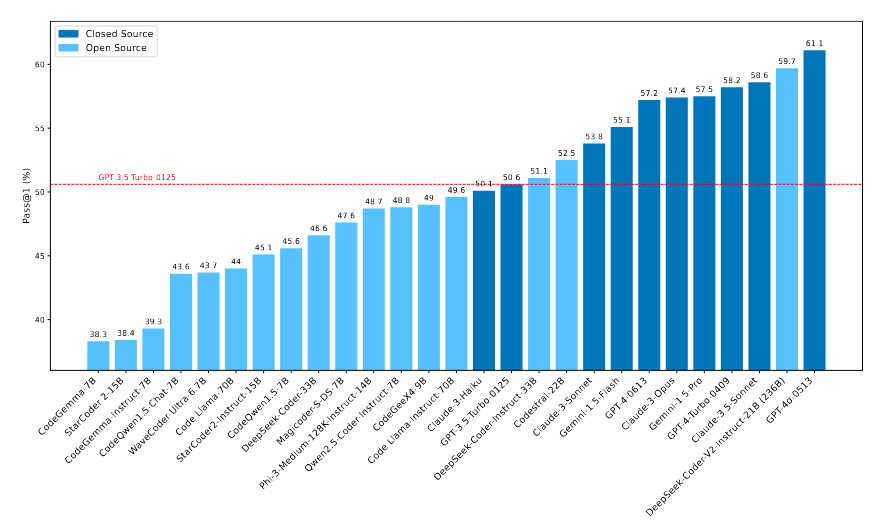
\includegraphics[width=0.8\textwidth]{./bilder/performance_comparison.png}
    \caption{Leistungsvergleich verschiedener Modellgrößen (nach Jiang et al. (2024), basierend auf 'A Survey on Large Language Models for Code Generation').}
    \label{fig:performance_comparison}
\end{figure}
In den letzten Jahren wurden mehrere Benchmarks und Evaluierungsdatensätze speziell für die Code-Generierung entwickelt. Beispiele dafür sind \emph{HumanEval}\cite{chen2021evaluatinglargelanguagemodels} und \emph{EvalPlus}\cite{evalplus}, die genutzt werden, um die Genauigkeit und Zuverlässigkeit von LLMs in verschiedenen Programmiersprachen zu testen. Erste Studien zeigen, dass LLMs einfache bis mittelschwere Aufgaben oft vollständig lösen können. Bei komplexeren oder sehr speziellen Aufgabenbereichen stoßen sie aber noch an ihre Grenzen\cite{NEURIPS2023_43e9d647}.
Obwohl LLMs in vielen Sprachen Code generieren können, hat sich Python als einer der Hauptfoki herauskristallisiert. Dies liegt an der weit verbreiteten Nutzung von Python in Wissenschaft und Industrie, insbesondere in den Bereichen Datenanalyse und Machine Learning. Die umfangreichen Bibliotheken wie NumPy, pandas und scikit-learn sind Teil der Trainingskorpora, wodurch LLMs häufig in der Lage sind, Standardroutinen oder Bibliotheksfunktionen korrekt anzuwenden\cite{chen2021evaluatinglargelanguagemodels}.

\subsection{Einführung Python}
\label{sec:Python}
TODO: ausführlicher
\subsubsection{Bedeutung und Bibliotheken}
Python ist dank seiner Syntax, aktiven Community und vielen hilfreichen Bibliotheken eine der am weitesten verbreiteten Sprachen für Datenanalyse. Ein paar der wichtigsten Bibliotheken, die in der Datenanalyse verwendet werden, sind:
\begin{itemize}
    \item \textbf{pandas} -- Datenstrukturen und -bearbeitung,
    \item \textbf{NumPy} -- numerische Berechnungen,
    \item \textbf{scikit-learn} -- Machine-Learning-Algorithmen,
    \item \textbf{Matplotlib} -- Visualisierung,
\end{itemize} 
Diese und weitere Bibliotheken ermöglichen eine effiziente Umsetzung datenanalytischer Projekte und werden bereits in LLM-Trainings berücksichtigt, wodurch generierter Code auf bekannte Funktionen zurückgreifen kann\cite{evalplus,chen2021codex}.

\subsubsection{Typische Schritte einer Datenanalyse}
Die Grundschritte einer klassischen Datenanalyse in Python enthält folgende Schritte:
\begin{enumerate}
    \item \textit{Datenimport} (z.\,B. CSV-Dateien, Datenbanken, APIs),
    \item \textit{Datenbereinigung} (fehlende Werte, Duplikate, Datentypen),
    \item \textit{Analyse und Visualisierung} (Statistiken, Plots),
\end{enumerate}
Im Rahmen dieser Arbeit wird untersucht, ob LLMs diese Schritte automatisieren können und an welchen Stellen manuell eingegriffen werden muss.

\subsection{Einführung automatisierte Code-Generierung}
\label{sec:AutoCode}

\subsubsection{Funktionsweise und Vorteile}
Automatisierte Code-Generierung mithilfe von LLMs basiert auf \emph{Prompts}, also Benutzeranfragen in natürlicher Sprache. LLMs haben hierbei die Möglichkeit sich flexibel an den vom Benutzer gegegeben Kontext anzupassen und können die natürliche Sprache in funktionsfähigen Code umwandeln. Ebenso müssen LLMs nicht spezifisch auf eine Aufgabe trainiert werden, aufgrund der großen Trainingsdaten, die ihnen zur Verfügung stehen\cite{chen2021evaluatinglargelanguagemodels}. Insbesondere für datenanalytische Aufgaben, bei denen standardisierte Skripte (z.\,B. für das Einlesen und Bereinigen von Daten) immer wieder benötigt werden, kann dies zu einer erheblichen Zeitersparnis führen und ermöglicht die Nutzung von LLMs auch für weniger erfahrene Personen, die nicht über tiefgreifende Programmierkenntnisse verfügen.

\subsubsection{Herausforderungen und Grenzen}
Trotz beeindruckender Fortschritte stößt die automatisierte Code-Generierung noch häufig an Grenzen\cite{nijkamp2023codegenopenlargelanguage,wang2021codet5identifierawareunifiedpretrained}:
\begin{itemize}
    \item \textbf{Komplexe Datenstrukturen}: LLMs zeigen teils Schwächen bei Aufgaben mit hochgradiger Komplexität oder spezifischem Wissen, wenn zu wenig Kontext durch den Nutzer gegeben wird\cite{nijkamp2023codegenopenlargelanguage,wang2021codet5identifierawareunifiedpretrained}.
    \item \textbf{Performanz}: Generierter Code ist nicht immer optimal hinsichtlich Laufzeit oder Speicherverbrauch\cite{wang2021codet5identifierawareunifiedpretrained}.
    \item \textbf{Wartbarkeit}: Kommentare, klare Code-Struktur und Dokumentation fehlen häufig.
    \item \textbf{Fehleranfälligkeit}: Auch Code, der vorerst funktionsfähig erscheint, kann immer noch Bugs oder Sicherheitslücken enthalten.
\end{itemize}
Wir präsent diese Herausforderungen in datenanalytischen Aufgaben sind, soll in den folgenden Kapiteln untersucht werden. Vor allem durch den Vergleich von generiertem und manuell geschriebenem Code lassen sich die Stärken und Schwächen von LLMs in der Datenanalyse besser einschätzen.

\subsection{Prompting mit Sprachmodellen}
\label{sec:prompting}

Mit dem Begriff \emph{Prompting} wird das Verfahren beschrieben, ein zuvor trainiertes Sprachmodell allein durch spezifische Eingabetexte (\emph{Prompts}) zu steuern, ohne weiteres trainieren des Modells. Im Gegensatz zur zuvor verbreiteten Vorgehensweise, ein vortrainiertes Modell für jede Aufgabe mit allen notwendigen Parametern komplett anzupassen, wird beim Prompting direkt auf das bereits eingearbeitete Wissen des Modells zurückgegriffen und steuert dadurch dessen Ausgabe durch passende Formulierungen\cite{liu2021pretrainpromptpredictsystematic}. Mit der Veröffentlichung großer Modelle wie GPT-3 zog dieses Vorgehen große Aufmerksamkeit auf sich, weil es diesen Modellen ermöglichte, durch spezifische Anweisungen in einer Prompt, komplexe Aufgaben zu lösen, wie Brown et al.(2020)\cite{brown2020languagemodelsfewshotlearners} zeigten.

\paragraph{Grundlegende Strategien}
\begin{itemize}
  \item \textbf{Zero-Shot, One-Shot und Few-Shot Prompting:}  
  Bei \emph{Zero-Shot} Prompting wird dem Modell lediglich eine Aufgabenbeschreibung gegeben, ohne Beispiele. Hierbei soll das Modell von alleine auf die richtige und gewünschte Lösung kommen. Bei \emph{One-Shot} wird dem genau ein Beispiel hinzugefügt, während \emph{Few-Shot} mehrere Demonstrationsbeispiele bereitstellt. Erste Arbeiten, wie jene von Brown et al.\cite{brown2020languagemodelsfewshotlearners}, zeigten, dass schon wenige Beispiele im Prompt teils große Leistungsunterschiede bewirken können.

  \item \textbf{Instruction-based Prompting:}  
  Anstatt nur Beispiele zu geben, werden präzise Anweisungen in Textform formuliert, wie beispielsweise \emph{„Fasse den Text in drei Sätzen zusammen.“}. Ouyang et al.(2022) führen dafür auch ihr Modell \emph{InstructGPT} ein, welches speziell darauf trainiert wurde, solche Anweisungen verlässlich und mit Berücksichtigung der Wünsche des Nutzers in korrekter Weise umzusetzen\cite{ouyang2022traininglanguagemodelsfollow}.

  \item \textbf{Chain-of-Thought Prompting:}  
  Hierbei wird das Modell dazu angewiesen Schrittweise vorzugehen und diese Zwischenschritte explizit auszugeben. Dadurch liefern Modelle oft bessere und eher nachvollziehbare Ergebnisse zurück, wie Wei et al.(2022) zeigen\cite{wei2023chainofthoughtpromptingelicitsreasoning}.
\end{itemize}


\section{LLMs in der Programmierung – aktueller Stand}
\label{sec:llms_programmierung}
Die Entwicklung von Large Language Models (LLMs) hat in den letzten Jahren nicht nur die Art und Weise, wie natürliche Sprache verarbeitet und generiert wird, verändert, sondern auch große Fortschritte in der automatisierten Code-Erstellung ermöglicht. Durch die Kombination aus leistungsstarken Modellarchitekturen wie Transformers, großen Mengen an Trainingsdaten und moderner Hardware haben LLMs heute eine große Präsemz in vielen Bereichen der Softwareentwicklung und Datenanalyse.
In diesem Kapitel werden die aktuellen Entwicklungen und verfügbaren Modelle vorgestellt. Außerdem wird ein Überblick über ihre Einsatzmöglichkeiten in der Softwareentwicklung und Datenanalyse gegeben. Zum Schluss werden wichtige Studien und Arbeiten zur Code-Generierung betrachtet, darunter etwa die von Chen et al. (2021) vorgestellte Arbeit zu Codex, einem Modell, das speziell für die automatisierte Programmierung entwickelt wurde\cite{chen2021evaluatinglargelanguagemodels} und die von Liu et al. (2023) veröffentlichte Arbeit zur Evaluation von generiertem Code mithilfe von \emph{EvalPlus}\cite{NEURIPS2023_43e9d647}.

\subsection{Überblick und Vergleich von verschiedenen LLMs}
Derzeit existiert eine Vielzahl an LLMs, darunter auch viele, die gezielt zur Code-Generierung entwickelt wurden. Zu den bekanntesten Beispielen zählen ChatGPT (GPTo1 als das modernste Modell), OpenAI Codex, Code Llama\cite{rozière2024codellamaopenfoundation}, StarCoder \cite{li2023starcodersourceyou}, CodeT5\cite{wang2021codet5identifierawareunifiedpretrained} oder CodeGen\cite{nijkamp2023codegenopenlargelanguage}.
\begin{figure}[H]
    \centering
    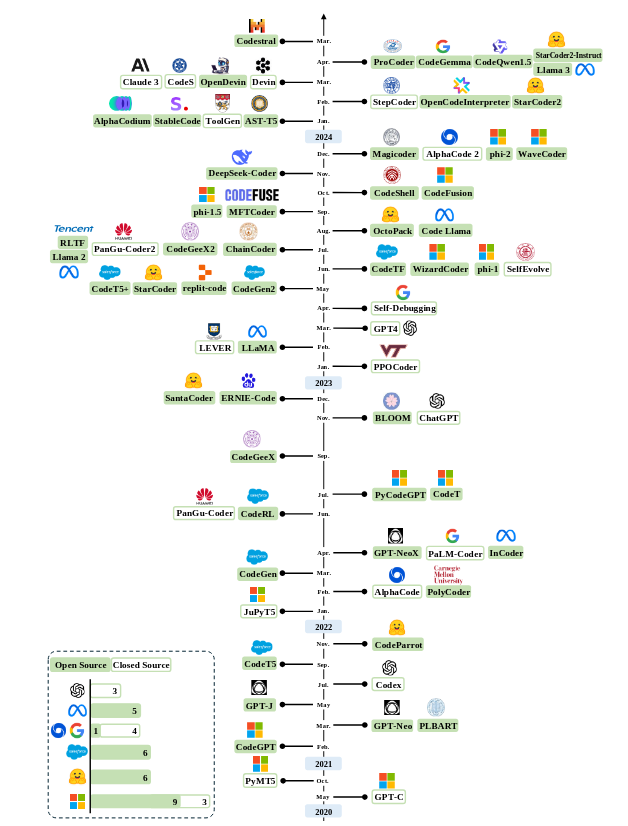
\includegraphics[width=0.8\textwidth]{./bilder/LLMs_for_coding.png}
    \caption{Chronologische Übersicht von Large Language Models für die Code Generierung der letzten Jahre (nach Jiang et al. (2024), basierend auf 'A Survey on Large Language Models for Code Generation').}
    \label{fig:llms_for_coding}
\end{figure}

Diese Modelle teilen sich häufig folgende Merkmale:
\begin{enumerate}
    \item \textbf{Transformer-Architektur}: Nahezu alle modernen LLMs beruhen auf dem Transformer-Modell.
    \item \textbf{Große Parameteranzahl}: Typische LLMs verfügen über eine Vielzahl an Parametern und benötigen entsprechend umfangreiche Trainingsdaten, zu denen in vielen Fällen öffentlich verfügbare Code-Repositories (z. B. GitHub) zählen\cite{chen2021evaluatinglargelanguagemodels}.
    \item \textbf{Breite Sprachenunterstützung}: Neben Python werden häufig Java, JavaScript und andere Programmiersprachen abgedeckt\cite{chen2021evaluatinglargelanguagemodels,jiang2024surveylargelanguagemodels}.
\end{enumerate}
Ein Vergleich der LLMs lässt sich anhand verschiedener Kriterien vornehmen:
\begin{itemize}
    \item \textbf{Größe und Trainingsdaten}: Modelle wie GPT-4 oder Code Llama sind mit einer Vielzahl an Code-Datensätzen trainiert und erreichen dadurch in Benchmarks eine hohe Erfolgsquote\cite{NEURIPS2023_43e9d647}.
    \item \textbf{Lizenz und Offenheit}: Neben proprietären Modellen, wie GitHub Copilot und ChatGPT, existieren mit Code Llama, StarCoder oder CodeGen auch Open Source Alternativen.
    \item \textbf{Spezialisierung}: Einige Modelle sind speziell auf Code-Generierung abgestimmt (z.B. Code Llama, StarCoder), wohingegen andere (z.B. ChatGPT) einen generellen Sprachkontext haben, um auch andere Fragen zu beantworten, der sich jedoch auch auf Code-Aufgaben anwenden lässt.
\end{itemize}

\subsection{Einsatzgebiete von LLMs in der Programmierung}
\label{sec:einsatzgebiete}
Die zunehmende Leistungsfähigkeit von Large Language Models (LLMs) ermöglicht es, Programmieraufgaben in diversen Bereichen zu automatisieren oder zu beschleunigen. Häufig genannte \emph{Einsatzgebiete} sind dabei:
\begin{itemize}
    \item \textbf{Code-Generierung}:
    Ermöglicht die Code-Generierung auf Grundlage von Beschreibungen aus natürlicher Sprache\cite{chen2021evaluatinglargelanguagemodels}. Ebenso bieten manche Modelle die Möglichkeit zu fertigen Funktionen Tests zu generieren, um dessen Funktionalität zu überprüfen.
    \item \textbf{Autovervollständigung}:  
    Integriert in Entwicklungsumgebungen wie Visual Studio Code können Tools wie GitHub Copilot repetitive Abläufe direkt im Code vervollständigen oder Vorschläge zur Vervollständigung von neu begonnenem Code liefern\cite{chen2021evaluatinglargelanguagemodels}.
    \item \textbf{Refactoring und Fehlersuche}:  
    Dank ihrer Kontextsensitivität können LLMs bestehenden Code analysieren und an einigen Stellen Möglichkeiten zur Optimierung oder Korrektur vorschlagen\cite{chen2021evaluatinglargelanguagemodels,wang2021codet5identifierawareunifiedpretrained}. Dadurch lassen sich Bugs, Redundanz und ineffiziente Code-Strukturen frühzeitig identifizieren und beheben.
    \item \textbf{Automatisierte Dokumentation und Code-Kommentierung}:  
    Viele Modelle bieten die Möglichkeit vorhandenen Code zu analysieren und dazu Kommentarblöcke oder gar ganze Dokumentationen zu erstellen\cite{wang2021codet5identifierawareunifiedpretrained,jiang2024surveylargelanguagemodels}.
\end{itemize}
Obwohl diese Einsatzgebiete großes Potenzial bieten, sind LLMs nicht frei von Fehlern. Gerade bei komplexen Entscheidungen zur Programm- und Codearchitektur können diese oft mit dem Level durch das menschliche Fachwissen nicht mithalten \cite{dhar2024llmsgeneratearchitecturaldesign}.

\subsection{Vergangene Studien und Arbeiten zur Code-Generierung}
\label{sec:vergangene_studien}

Die Forschung zur automatisierten Code-Generierung hat in den letzten Jahren eine rasante Entwicklung erlebt, wobei Arbeiten aus den Bereichen \emph{Software Engineering}, \emph{Large Language Models} und \emph{Machine Learning} zusammenfließen. Jiang et al. (2024) haben in ihrer Arbeit "A Survey on Large Language Models for Code Generation" eine Übersicht über die Entwicklung der veröffentlichten Arbeiten zu LLMs und Software Engineering erstellt, welche in Abbildung \ref{fig:entwicklung_paper} dargestellt ist.
\begin{figure}[H]
    \centering
    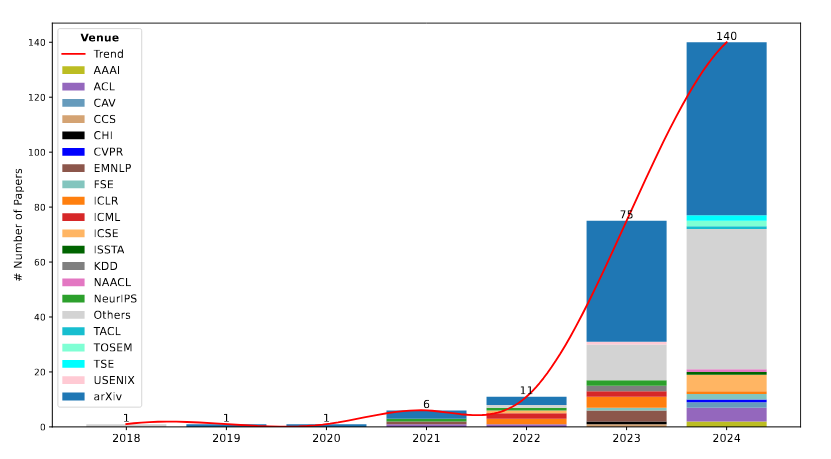
\includegraphics[width=0.8\textwidth]{./bilder/entwicklung_paper.png}
    \caption{Übersicht der Verteilung von veröffentlichten Arbeiten zu LLMs und Software Engineering der letzten Jahren (nach Jiang et al. (2024), basierend auf 'A Survey on Large Language Models for Code Generation').}
    \label{fig:entwicklung_paper}
\end{figure}

Im Folgenden werden einige vergangene Studien/Arbeiten zur Code Generierung mit LLMs vorgestellt:
\begin{enumerate}
    \item \textbf{"Is Your Code Generated by ChatGPT Really Correct? Rigorous Evaluation of Large Language Models for Code Generation"} von Liu et al. (2023) \cite{NEURIPS2023_43e9d647}:\\
    In diesem Paper wird untersucht, wie korrekt der von LLMs wie ChatGPT, Code Llama etc. generierte Code ist. Dafür wird \emph{EvalPlus} eingeführt. Dies ist ein neues Evaluierungsframework, das bestehende Testdatensätze wie \emph{HumanEval} durch weitere automatisierte Testfälle erweitert. Hier kommen Liu et al. zu dem Ergebnis, dass bisher viele Fehler in generiertem Code nicht erkannt wurden, wodurch die Modelle in ihrer Leistung überschätzt wurden. Die Autoren weisen darauf hin, wie wichtig umfassendene Tests sind, um die tatsächliche Funktionalität der LLMs für die Codegenerierung zu bewerten.
TODO: Vielleicht Grafik der Ergebnisse einfügen
    \item \textbf{Evaluating Large Language Models Trained on Code} von Chen et al. (2021) \cite{chen2021evaluatinglargelanguagemodels}:\\
    In diesem Paper wird Codex vorgestellt. Dies ist ein LLM, das speziell auf öffentlich verfügbarem Code von Github trainiert wurde, um dessen Fähigkeiten Python Code zu schreiben zu analysieren. Dies wird mithilfe des HumanEval-Datensatzes untersucht. Hierbei soll im genauen Python-Code aus Docstrings generiert und dieser dann bewertet werden. Die Ergebnisse zeigen, dass Codex im Vergleich zu anderen Modellen wie GPT-3 deutlich besser abschneidet, jedoch bei komplexeren Aufgaben seine Grenzen erreicht. Eine mehrfach wiederholte Lösungsgenerierung verbessert die Erfolgsrate, was das Potenzial ihres Ansatzes verdeutlicht.

    \item \textbf{A Survey on Large Language Models for Code Generation} von Jiang et al. (2024) \cite{jiang2024surveylargelanguagemodels}:\\
    Dieses Paper gibt einen allgemeinen und umfassenden Überblick über den aktuellen Forschungsstand zu LLMs für die Codegenerierung. Es greift Themen wie Datenaufbereitung, Modellarchitekturen und Benchmarks auf. Zudem werden Herausforderungen, wie die praktische Einführung und ethische Fragen diskutiert. Die Autoren leiten sich wichtige Forschungsfragen ab und verdeutlichen, dass LLMs in der Codegenerierung große Fortschritte gemacht haben, aber es weiterhin Potenzial zur Optimierung gibt.

    \item \textbf{Evaluating Language Models for Efficient Code Generation} von Liu et al. (2024) \cite{liu2024evaluating}
    Auch in dieser Arbeit von Jiawei Liu wird die Effizienz von Code untersucht, welcher von LLMs generiert wird. Hierbei mit Fokus auf Performance und Ressourcennutzung. Dafür wird \emph{Differential Performance Evaluation (DPE)} entwickelt und der \emph{EvalPerf}-Benchmark eingeführt. Dieser enthält komplexere Programmieraufgaben als der zuvor eingeführt \emph{EvalPlus}. Hier kommt man zu dem Entschluss, dass größere Modelle nicht automatisch auch effizienteren Code erzeugen. Stattdessen werden Effizienz und Korrektheit des Codes durch \emph{Instruction Tuning}(gezieltes Trainieren des Modells, um besser auf Anweisungen in natürlicher Sprache zu reagieren) verbessert.
\end{enumerate}
Zusammenfassend zeigen die genannten Studien, dass LLMs zwar großes Potenzial zur automatisierten Code Generierung besitzen, sie aber immer noch Probleme aufweisen und menschliche Entwickler nicht komplett ersetzen können. Besonders bei komplexeren Aufgaben, spezifischen Anforderungen oder Fragen zur Softwarearchitektur stoßen sie an ihre Grenzen.

\section{Ausgangsdaten und Testfallspezifikation}
\subsection{Überblick und Reduktion der Datengrundlage}
Die Datengrundlage für die empirische Untersuchung bilden Kriminalitätsstatistiken (sogenannte \emph{Fallzahlen}) der Stadt Berlin\cite{opendataberlin}. Die zugehörige Excel-Datei umfasst mehrere Sheets, jeweils zu den Jahren 2014--2023. Darin sind die Straftaten pro Bezirk (bzw. Ober- und Unterbezirke) aufgelistet. In der Ursprungsform gliedert sich die Tabelle wie folgt:
\begin{itemize}
    \item \textbf{Oberbezirk}: Enthält aggregierte Zahlen der jeweiligen Unterbezirke.
    \item \textbf{Unterbezirke}: Ausführlichere Aufschlüsselung der Straftaten innerhalb des Oberbezirks.
    \item \textbf{Spalten mit Straftat-Kategorien}: u.\,a. \enquote{Straftaten insgesamt}, \enquote{Körperverletzungen}, \enquote{Diebstahl}, \dots
\end{itemize}

Für die weitere Analyse wird jedoch nur auf \emph{Oberbezirks}-Daten zurückgegriffen. Die Unterbezirke werden \textbf{nicht} berücksichtigt, um die Komplexität zu reduzieren und das Fokusgebiet auf obergeordnete Bezirke zu legen. Ziel ist eine übersichtlichere Zusammenfassung, bei der \enquote{Oberbezirk} die wichtigste Bezugsgröße ist.

\subsection{Umwandlung in Pandas DataFrames}
Jedes Jahr (bzw. jedes Sheet) soll in einer separaten \texttt{pandas}-DataFrame-Tabelle abgebildet werden. Dies geschieht folgendermaßen:
\begin{enumerate}
    \item \textbf{Reduzieren der Datengrundlage}: Entfernen der Unterbezirke, um nur die Oberbezirke zu behalten.
    \item \textbf{Bereinigung und Umbenennung}: Unnötige Spalten werden entfernt, Spaltennamen ggf. standardisiert (z.\,B. \enquote{Bezirk}, \enquote{Straftaten\_insgesamt}).
    \item \textbf{Einlesen der Excel-Sheets}: Mit \texttt{pandas.read\_excel(...)} wird jede Jahres-Tabelle eingelesen.
    \item \textbf{Speicherung in DataFrame}: Pro Sheet entsteht ein bereinigtes und vereinheitlichtes DataFrame.
\end{enumerate}

\subsection{Testfälle und Vorgehen}
Insgesamt sind vier Testfälle definiert, die unterschiedliche Aspekte der Datenanalyse abdecken. Für jeden Testfall werden \textbf{15 Ausführungen} erzeugt, wobei drei verschiedene Prompting-Strategien (jeweils fünf Wiederholungen) zum Einsatz kommen:
\begin{itemize}
    \label{itemize:promptingstrategien}
    \item \textbf{Strategie A: Prompt wie ein \enquote{normaler User}}\\
    Hier wird eine einfache, natürlichsprachliche Anfrage formuliert, ohne viele zusätzliche Informationen.
    \item \textbf{Strategie B: Prompt mit Metadaten}\\
    In diesem Ansatz werden neben der eigentlichen Anfrage auch relevante Details wie Spaltennamen oder Strukturhinweise explizit übergeben.
    \item \textbf{Strategie C: Prompt mit \emph{Chain of Thought}}\\
    Das Modell erhält schrittweise Gedankenanstöße oder Zwischenlogik (z.\,B. \enquote{Zuerst filtern, dann sortieren, ...}), um den Code schrittweise aufzubauen und zu erklären.
\end{itemize}

\subsubsection{Testfall 1: Sortierung und Ausgabe der Fallzahlen 2023}
\label{subsec:tf1}
\paragraph{Zielsetzung:}
Die Daten des Jahres 2023 (\texttt{Fallzahlen\_2023}) sollen nach der Spalte \enquote{Straftaten insgesamt} sortiert und anschließend in einem \texttt{pandas}-DataFrame ausgegeben werden.

\paragraph{Vorgehen:}
\begin{enumerate}
    \item Einlesen der \texttt{Fallzahlen\_2023}.
    \item Extraktion der relevanten (Ober-)Bezirke.
    \item Sortierung nach \texttt{Straftaten\_insgesamt} in absteigender oder aufsteigender Reihenfolge.
    \item Ausgabe als \texttt{pandas} DataFrame.
\end{enumerate}

\paragraph{Erwartete Ausgabe:}
Ein DataFrame mit mindestens folgenden Spalten:
\begin{center}
\begin{tabular}{l|l}
\textbf{Bezirk} & \textbf{Straftaten\_insgesamt} \\
\hline
\textit{(z.\,B. Mitte)} & \textit{(z.\,B. 82\,000)} \\
\textit{(z.\,B. Neukölln)} & \textit{(z.\,B. 50\,000)} \\
... & ...
\end{tabular}
\end{center}
Zusätzlich können weitere Spalten (z.\,B. Raub, Diebstahl) enthalten sein, sofern sie nicht entfernt wurden.

\subsubsection{Testfall 2: Join aller Tabellen und \enquote{Bezirks-Topwert}}
\paragraph{Zielsetzung:}
Alle DataFrames von 2014--2023 sollen \emph{vereint} werden (Join), sodass die \textbf{Summe der Straftaten aller Jahre} pro Bezirk ermittelbar ist. Anschließend werden die Bezirke nach \enquote{den meisten Straftaten insgesamt} sortiert ausgegeben.

\paragraph{Vorgehen:}
\begin{enumerate}
    \item Einlesen und Bereinigung der einzelnen DataFrames (2014--2023).
    \item Zusammenführen nach dem \texttt{Bezirk}-Merkmal.
    \item Aggregation der \enquote{Straftaten\_insgesamt} pro Jahr zu einer Gesamtzahl über alle Jahre.
    \item Ermittlung und Ausgabe der \texttt{Bezirke} sortiert nach den Summenwerten.
\end{enumerate}

\paragraph{Erwartete Ausgabe:}
Ein DataFrame mit mindestens folgenden Spalten:
\begin{center}
\begin{tabular}{l|l}
\textbf{Bezirk} & \textbf{Straftaten\_insgesamt 2014-2023} \\
\hline
\textit{(z.\,B. Mitte)} & \textit{(z.\,B. 820\,000)} \\
\textit{(z.\,B. Neukölln)} & \textit{(z.\,B. 560\,000)} \\
... & ...
\end{tabular}
\end{center}

\subsubsection{Testfall 3: Prozentuale Verteilung der Straftaten}
\paragraph{Zielsetzung:}
Für ein ausgewähltes Jahr (etwa 2023) soll ermittelt werden, welcher Anteil aller Berliner Straftaten auf die jeweiligen Bezirke entfällt.

\paragraph{Vorgehen:}
\begin{enumerate}
    \item Einlesen des relevanten Sheets (z.\,B. \texttt{Fallzahlen\_2023}).
    \item Berechnung des Anteils pro Bezirk: 
    \[
       \text{Prozent} = \frac{\text{Straftaten\_insgesamt pro Bezirk}}{\text{Straftaten\_Gesamtsumme}} \times 100 
    \]
    \item Ausgabe als DataFrame mit Spalten wie \enquote{Bezirk}, \enquote{Straftaten\_insgesamt}, \enquote{Anteil\_\%}.
\end{enumerate}

\paragraph{Erwartete Ausgabe:}
Ein DataFrame, bei dem jede Zeile einen \texttt{Bezirk} darstellt und mindestens folgende Spalten beinhaltet:
\begin{center}
\begin{tabular}{l|l|l}
\textbf{Bezirk} & \textbf{Straftaten\_insgesamt} & \textbf{Anteil\_(\%)} \\
\hline
\textit{Mitte} & \textit{82\,000} & \textit{(z.\,B. 24,1\%)} \\
\textit{Neukölln} & \textit{50\,000} & \textit{(z.\,B. 14,7\%)} \\
... & ... & ...
\end{tabular}
\end{center}

\subsubsection{Testfall 4: Zeitreihe über die Jahre 2014--2023}
\paragraph{Zielsetzung:}
Ausgabe der \textbf{prozentualen Entwicklung} (bezogen auf \emph{Berlin insgesamt}) der \texttt{Straftaten\_insgesamt} pro Jahr, bezogen auf das Vorjahr. Damit soll ersichtlich werden, wie sich das Gesamtaufkommen an Straftaten im Zeitverlauf verändert hat. 

\paragraph{Vorgehen:}
\begin{enumerate}
    \item Einlesen sämtlicher Jahres-Sheets.
    \item Addition sämtlicher Bezirkswerte für jedes Jahr, um die Gesamtzahl an Straftaten je Jahr zu erhalten.
    \item Direkter Vergleich \enquote{prozentuale Änderung} zum Vorjahr.
    \item Ausgabe eines \texttt{pandas} DataFrames als Zeitreihe.
\end{enumerate}

\paragraph{Erwartete Ausgabe:}
Ein DataFrame mit mindestens zwei Spalten:
\begin{center}
\begin{tabular}{l|l}
\textbf{Jahr} & \textbf{Straftaten\_Veränderung\_(\%) zu Vorjahr} \\
\hline
2014 & 0\% (Basiswert) \\
2015 & +3,5\% \\
2016 & -1,2\% \\
... & ...
\end{tabular}
\end{center}

\section{Methodik}
\label{sec:methodik}
TODO: noch mehr ausschreiben

\subsection{Vorgehensweise der Untersuchung}
    In der Untersuchung soll geprüft werden, inwieweit Large Language Models in der Lage sind gängige Datenanalyse-Schritte auf Grundlage eines gegebenen Datensatzes durchzuführen. Hierbei wird ChatGPT als aktueller Marktführer mit dem Sprachmodell GPTo1, welches das neueste Modell ist, verwendet. Ebenso gilt es herauszufinden wie qualitativ und effizient diese Lösung ist. Hierbei bezieht es sich auf die Forschungsfragen aus Kapitel \ref{sec:forschungsfragen}.
    Für die Vorgehensweise hierbei wird zuerst der verwendete Datensatz von Berlin Open Data an das Modell übergeben und dazu eine Prompt verfasst. Diese Prompts können in Kapitel \ref{sec:testfaelle} eingesehen werden.
    Im Anschluss durchläuft der Code mehrere Tests und manuelle Analysen um die Qualität und Effizienz des generierten Codes zu bewerten. Die genauen Auswertungskriterien sind in Kapitel \ref{sec:auswertungskriterien} aufgeführt.
    Die Ergebnisse der Auswertung werden in Kapitel \ref{sec:auswertung} detailliert dargestellt und auch mit den Ergebnissen anderer Arbeiten, wie etwa von Chen et al. (2021)\cite{chen2021evaluatinglargelanguagemodels} und Liu et al. (2023)\cite{NEURIPS2023_43e9d647} verglichen.

\subsection{Testfälle der Datenanalyse}
\label{sec:testfaelle}
\subsubsection{Testfall 1}
    Im ersten Testfall soll der Datensatz nach einer gewissen Spalte sortiert werden. Die Begründung hierfür ist, dass dies eine sehr einfache, aber auch sehr häufig aufkommende Datenanalyse-Aufgabe ist und somit einen guten Einstieg in die Untersuchung darstellt. Die Prompts für diese Aufgabe lauten:
    \begin{itemize}
        \item \textbf{Zero-Shot Prompting}: \emph{Ich habe eine Excel Datei mit dem Namen 'Fallzahlen.xlsx'. Hier ist der Inhalt des Sheets 'Fallzahlen\_2023': \texttt{[DataFrame]}. Erstelle mir ein Skript in Python, das die Daten aus der Excel-Datei einliest, nach den Straftaten insgesamt der Bezirke sortiert und in einem Dataframe speichert.}
        \item \textbf{Instruction Prompting}: \emph{Ich habe eine Excel Datei mit dem Namen 'Fallzahlen.xlsx'. Hier ist der Inhalt des Sheets 'Fallzahlen\_2023': \texttt{[DataFrame]}. Erstelle mir ein Skript in Python, das die Daten aus der Excel-Datei einliest, nach der Spalte 'Straftaten\_insgesamt' der Bezirke sortiert und in einem Pandas Dataframe speichert. Die Zeilen mit den LOR-Schlüsseln 999900 und 999999 sollen bei der Sortierung außer Acht gelassen werden, da es sich bei diesen nicht um Bezirke handelt.}
        \item \textbf{Chain-of-Thought Prompting}: \emph{Ich habe eine Excel Datei mit dem Namen 'Fallzahlen.xlsx'. Der Inhalt des Sheets ist als pandas DataFrame \texttt{[DataFrame]} gegeben. Bitte erstelle mir ein Python-Skript, das die folgenden Schritte ausführt:\\1. Lies die Daten des Sheets 'Fallzahlen\_2023' der Excel-Datei 'Fallzahlen.xlsx' ein.\\2. Sortiere die Daten nach der Spalte 'Straftaten\_insgesamt' absteigend. Zur Sortierung sollen die Zeilen mit den LOR-Schlüsseln 999900 und 999999 nicht beachtet werden, da es sich bei diesen nicht um Bezirke handelt. Sie sollen aber am Ende des Dataframes stehen bleiben.\\3. Speichere das Ergebnis der Sortierung in einem Pandas Dataframe ab.\\Achte darauf, dass das Skript robust ist und potentielle Fehler, wie fehlende Spalten berücksichtigt.}
    \end{itemize}

\subsubsection{Testfall 2 Verbund und Aggregation}
    Für den zweiten Testfall sollen die Tabellen der Excel Datei durch einen Join zusammengeführt und dann die Bezirke nach den Straftaten insgesamt von allen Jahren kombiniert geliefert werden. Die Prompts für diese Aufgabe lauten:
    \begin{itemize}
        \item \textbf{Zero-Shot Prompting}: \emph{Ich habe eine Excel Datei mit dem Namen 'Fallzahlen.xlsx'. Erstelle mir ein Python Skript, das die Daten aller Sheets zusammenliest, sie nach der Anzahl der Straftaten insgesamt pro Bezirk sortiert und in einem Pandas DataFrame speichert. Hier sind die Daten eines der Sheets als Beispiel: \texttt{[DataFrame]}}
        \item \textbf{Instruction Prompting}: \emph{Ich habe eine Excel Datei mit dem Namen 'Fallzahlen.xlsx'. Erstelle mir ein Python Skript, das die Daten der einzelnen Bezirke (Zeilen) aller Sheets mit einem Join zusammenfügt, sie nach der akkumulierten Spalte 'Straftaten\_insgesamt' pro Bezirk sortiert und in einem Pandas DataFrame speichert. Die Zeilen mit den LOR-Schlüsseln 999900 und 999999 sollen bei der Sortierung nicht beachtet werden, da es sich hierbei nicht um Bezirke handelt. Hier sind die Daten eines der Sheets als Beispiel: \texttt{[DataFrame]}}
        \item \textbf{Chain-of-Thought Prompting}: \emph{Ich habe eine Excel Datei mit dem Namen 'Fallzahlen.xlsx'. Erstelle mir ein Python Skript, das folgende Anforderungen erfüllen soll:\\ 1. Die Excel-Datei einlesen und die Sheets als DataFrames speichern.\\ 2. Die DateFrames der einzelnen Sheets zusammen joinen, sodass pro Zeile (jede Zeile ist ein eigener Bezirk) der akkumulierte Wert der einzelnen Straftaten steht.\\ 3. Das neue gejointe DataFrame nach der Spalte 'Straftaten\_insgesamt' sortieren. Für die Sortierung sollen die Zeilen mit den LOR-Schlüsseln 999900 und 999999 nicht beachtet werden, da es sich hierbei nicht um Bezirke handelt. Sie sollen aber am Ende des DataFrames stehen bleiben.\\ 4. Das sortierte Pandas DataFrame zurückgeben.\\ Hier ist der Inhalt eines der Sheets als Beispiel: \texttt{[DataFrame]}}
    \end{itemize}

\subsubsection{Testfall 3}
    Im dritten Testfall soll das Sprachmodell die prozentualen Anteile der gesamten Straftaten der Bezirke von ganz Berlin berechnen. Die Prompts für diese Aufgabe lauten:
    \begin{itemize}
        \item \textbf{Zero-Shot Prompting}: \emph{Ich habe eine Excel Datei mit dem Namen 'Fallzahlen.xlsx'. Erstelle mir ein Python Skript, welches den prozentualen Anteil der gesamten Straftaten der einzelnen Bezirke von den gesamten Straftaten von ganz Berlin berechnet. Hier ist der Inhalt des Sheets 'Fallzahlen\_2023': \texttt{[DataFrame]}}
        \item \textbf{Instruction Prompting}: \emph{Ich habe eine Excel Datei mit dem Namen 'Fallzahlen.xlsx'. Erstelle mir ein Python Skript, welches den prozentualen Anteil der einzelnen Bezirke von ganz Berlin für die Spalte 'Straftaten\_insgesamt' berechnet. Jede Zeile der Tabelle ist ein einzelner Bezirk und 'Berlin (PKS gesamt)' ist die Gesamtanzahl von ganz Berlin. Hier ist der Inhalt des Sheets 'Fallzahlen\_2023': \texttt{[DataFrame]}}
        \item \textbf{Chain-of-Thought Prompting}: \emph{Ich habe eine Excel Datei mit dem Namen 'Fallzahlen.xlsx'. Erstelle mir ein Python Skript, welches folgende Anforderungen erfüllt:\\ 1. Die Excel-Datei einlesen\\ 2. Die Tabelle als Pandas DataFrame speichert\\ 3. Überprüfen, ob die notwendigen Spalten 'Bezirke' und 'Straftaten\_insgesamt' vorhanden sind\\ 4. Finde die Gesamtzahl der Straftaten für ganz Berlin in der Zeile mit dem Bezirk 'Berlin (PKS gesamt)'\\ 5. Berechne den prozentualen Anteil der einzelnen Bezirke von ganz Berlin für die Spalte 'Straftaten\_insgesamt'\\ 6. Das Ergebnis als DataFrame zurückgeben\\ Hier ist der Inhalt des Sheets 'Fallzahlen\_2023': \texttt{[DataFrame]}}
    \end{itemize}

\subsubsection{Testfall 4}
    Im vierten Testfall sollen die Skripte eine Zeitreihe der prozentualen Veränderung der gesamten Straftaten von ganz Berlin als Pandas Dataframe erstellen. Die Prompts für diese Aufgabe lauten:
    \begin{itemize}
        \item \textbf{Zero-Shot Prompting}: \emph{Ich habe eine Excel Datei mit dem Namen 'Fallzahlen.xlsx'. Erstelle mir ein Python Skript, das die Daten aller Sheets analysiert und eine Zeitreihe mit der prozentualen Veränderung zum jeweiligen Vorjahr der gesamten Straftaten von ganz Berlin als Pandas Dataframe erstellt.\\Hier sind die Daten eines der Sheets als Beispiel: \texttt{[DataFrame]}}
        \item \textbf{Instruction Prompting}: \emph{Ich habe eine Excel Datei mit dem Namen 'Fallzahlen.xlsx'. Erstelle mir ein Python Skript, das die Daten aller Sheets analysiert und eine Zeitreihe mit der prozentualen Veränderung der Spalte "Straftaten\_insgesamt" zum jeweiligen Vorjahr von der Zeile "Berlin (PKS gesamt)" als Pandas Dataframe erstellt. Die Sheets folgen der Namensgebung 'Fallzahlen\_2014', 'Fallzahlen\_2015', etc.\\Hier sind die Daten eines der Sheets als Beispiel: \texttt{[DataFrame]}}
        \item \textbf{Chain-of-Thought Prompting}: \emph{Ich habe eine Excel-Datei mit dem Namen 'Fallzahlen.xlsx'. Diese Datei enthält mehrere Sheets, die nach dem Muster 'Fallzahlen\_2014', 'Fallzahlen\_2015', usw. benannt sind. Jedes Sheet enthält Daten, darunter eine Spalte namens 'Straftaten\_insgesamt'. Erstelle mir ein Python Skript mit den folgenen Schritten:\\ 1. Lese alle Sheets der Excel-Datei ein und speichere jedes Sheet in einem separaten Pandas DataFrame.\\ 2. Extrahiere den Wert der Spalte 'Straftaten\_insgesamt' für die Zeile 'Berlin (PKS gesamt)' aus jedem DataFrame.\\ 3. Berechne die prozentuale Veränderung des Werts 'Straftaten\_insgesamt' zum jeweiligen Vorjahr.\\4. Speichere die Ergebnisse in einem neuen Pandas DataFrame, das die Jahre und die prozentuale Veränderung enthält.\\Hier sind die Daten eines der Sheets als Beispiel: \texttt{[DataFrame]}}
    \end{itemize}


\subsection{Auswertungskriterien}
\label{sec:auswertungskriterien}
    Korrektheit des Codes und der Ergebnisse, Performance des Codes im Bezug auf Laufzeit und Ressourcennutzung, Qualität des Codes (Struktur des Codes, Kommentare/Dokumentation, verwendete Libraries), Wartbarkeit und ist der Code erweiterbar.\\

    Die Auswertung der generierten Python Skripte erfolgt anhand der in Kapitel \ref{sec:forschungsfragen} definierten Kriterien. Um die Korrektheit des Codes zu messen wird das Pass@k Verfahren verwendet, dabei steht "k" für die Anzahl der ausgeführten Versuche pro Testfall. In diesem Experiment beschränke ich mich auf k=10, um eine gute Balance zwischen Genauigkeit und Rechenzeit zu finden. Bei diesem Verfahren ergibt sich als Ergebnis ein Prozentsatz über die Anzahl der erfolgreichen Versuche. Die ausgeführten Versuche werden anschließend in erfolgreich und nicht erfolgreich unterteilt und getrennt genauer betrachtet. Um zu entscheiden, ob ein Versuch erfolgreich war, werden Tests definiert, welche das Ergebnis und den Code selbst prüfen. Im Code wird dabei darauf geachtet, welche Bibliotheken, Funktionen und Pandas Dataframes benutzt wurden.
    In der genaueren Analyse des Codes wird bei den nicht erfolgreichen Versuchen wird untersucht, warum der Code nicht korrekt ausgeführt wurde und was für Verbesserungen vorgenommen werden können. Bei den erfolgreichen Versuchen hingegen wird analysiert, wie der Code strukturiert ist, ob er gut dokumentiert ist, ob er erweiterbar ist und wie die Laufzeit und Ressourcennutzung des Codes abschneidet.

\subsection{Verwendete Tools}
    \begin{enumerate}
        \item \textbf{Large Language Model}: Als Large Language Model wird ChatGPT mit GPTo1-mini verwendet, da ChatGPT als aktueller Marktführer gilt und GPTo1-mini das neueste und leistungsfähigste Modell ist, welches mit der OpenAI API verfügbar ist.
        TODO Libraries hinzufügen
    \end{enumerate}

\section{Auswertung der Python-Code-Generierung zur Datenanalyse durch LLMs}
\label{sec:auswertung }
\subsection{Testfall 1: Sortierung und Ausgabe der Fallzahlen 2023}
\label{subsec:auswertung_testfall1 }
    
Im ersten Testfall wurde ein Python-Skript generiert, das die Excel-Tabelle \enquote{Fallzahlen\_2023} nach der Anzahl der Straftaten insgesamt in 2023 sortieren sollte. Hierfür wurden drei verschiedene Prompting-Strategien (A, B, C\ref{itemize:promptingstrategien}) verwendet, wobei jede Strategie fünfmal ausgeführt wurde. Die wichtigsten Beobachtungen sind:
    
\paragraph{Erfolgsquote (Pass@15):}
\begin{itemize}
    \item \textbf{Prompt 1 (Zero-Shot Prompting)}: Alle fünf Ausführungen waren teils erfolgreich. Die Daten wurden zwar korrekt sortiert, jedoch wurden die Zeilen mit den LOR-Schlüsseln 999900 und 999999 (die nicht zu den Bezirken gehören) in die Sortierung einbezogen, was nicht der gewünschten Anforderung entsprach.
    \item \textbf{Prompt 2 (Instruction Prompting)}: Alle fünf Ausführungen waren teils erfolgreich. Die Zeilen mit den LOR-Schlüsseln 999900 und 999999 wurden korrekt aus der Sortierung ausgeschlossen, jedoch wurden sie vollständig aus dem DataFrame entfernt, was ebenfalls nicht der gewünschten Anforderung entsprach.
    \item \textbf{Prompt 3 (Chain of Thought Prompting)}: Alle fünf Ausführungen waren erfolgreich. Die Skripte sortierten die Daten korrekt nach der Spalte \enquote{Straftaten\_insgesamt} und behielten dabei die Zeilen mit den LOR-Schlüsseln 999900 und 999999 am Ende des DataFrames, wie gewünscht.
\end{itemize}
Berücksichtigt man die Teilerfolge als fehlgeschlagen, ergibt sich ein \textbf{Pass@15 von 33\%} (5 von 15 Ausführungen waren vollständig erfolgreich). Betrachtet man die Teilerfolge jedoch als erfolgreich, ergibt sich ein \textbf{Pass@15 von 100\%} (15 von 15 Ausführungen waren teils erfolgreich).
    
\paragraph{Korrektheit und typische Fehlerquellen:}
\begin{itemize}
    \item \textbf{Prompt 1}: Der Hauptfehler lag darin, dass die Zeilen mit den LOR-Schlüsseln 999900 und 999999 (also keinem Bezirk zuzuordnende Straftaten und Berlin gesamt) in die Sortierung einbezogen wurden. Dies führte dazu, dass die Sortierung nicht den Anforderungen entsprach, da diese Zeilen nicht zu den Bezirken gehören.
    \item \textbf{Prompt 2}: Hier wurden die Zeilen mit den LOR-Schlüsseln 999900 und 999999 (also keinem Bezirk zuzuordnende Straftaten und Berlin gesamt) zwar korrekt aus der Sortierung ausgeschlossen, jedoch wurden sie vollständig aus dem DataFrame entfernt, was ebenfalls nicht den Anforderungen entsprach.
    \item \textbf{Prompt 3}: Diese Strategie war die einzige, die alle Anforderungen erfüllte. Die Daten wurden korrekt sortiert, und die Zeilen mit den LOR-Schlüsseln 999900 und 999999 (also keinem Bezirk zuzuordnende Straftaten und Berlin gesamt) wurden am Ende des DataFrames belassen.
\end{itemize}
    
\paragraph{Performance und Ressourcenverbrauch:}
\begin{itemize}
    \item Die Laufzeit betrug bei allen erfolgreichen und teils erfolgreichen Skripten nur wenige Zehntelsekunden (zwischen 0,49 und 0,56 Sekunden).
    \item Der Speicherverbrauch bewegte sich bei rund 150,MB \emph{Maximum Resident Set Size}, was für diesen kleinen Datensatz sehr effizient ist.
    \item Die CPU-Auslastung lag bei allen Ausführungen zwischen 445\% und 498\%, was auf eine effiziente Nutzung der verfügbaren Ressourcen hinweist.
\end{itemize}
    
\paragraph{Codequalität und Wartbarkeit:}
\begin{itemize}
    \item \textbf{Struktur}: Die meisten Skripte bestanden aus wenigen, übersichtlichen Schritten: \emph{Daten einlesen}, \emph{Spalte bereinigen/umbenennen}, \emph{sortieren}, \emph{Datei abspeichern}. Die Skripte von Prompt 3 waren dabei am strukturiertesten und enthielten zusätzliche Schritte zur Fehlerbehandlung und Robustheit.
    \item \textbf{Dokumentation}: Die Skripte waren in der Regel gut kommentiert und erklärten die Schritte und die Funktionsweise. Dies war insbesondere bei den Skripten von Prompt 3 der Fall, die zusätzliche Kommentare zur Fehlerbehandlung und zur Logik der Sortierung enthielten.
    \item \textbf{Erweiterbarkeit}: Die Skripte von Prompt 3 waren am einfachsten zu erweitern, da sie bereits eine robuste Fehlerbehandlung enthielten und die Logik der Sortierung klar dokumentiert war. Die Skripte von Prompt 1 und 2 waren weniger robust, da sie keine Fehlerbehandlung für mögliche Änderungen in den Spaltennamen oder Datenstrukturen enthielten.
\end{itemize}
    
\paragraph{Fazit zu Testfall 1:}
Die Ergebnisse zeigen, dass die \textbf{Prompting-Strategie C (Chain of Thought)} die zuverlässigste Methode zur Generierung von Python-Code für die Sortierung eines Excel-Datensatzes ist. Diese Strategie lieferte in allen Fällen korrekte und robuste Skripte, die den Anforderungen entsprachen. Die Strategien A und B waren weniger zuverlässig, da sie entweder die Sortierung nicht korrekt durchführten oder die Daten unvollständig zurückgaben.

In Bezug auf \textbf{Performance} gab es keine Probleme, und alle Skripte waren effizient. Die Codequalität war bei den Skripten von Prompt 3 am höchsten, da sie gut dokumentiert und robust waren. Für produktive Einsätze ist daher die Verwendung von \textbf{Chain of Thought}-Prompts zu empfehlen, um sicherzustellen, dass der generierte Code den Anforderungen entspricht und leicht erweitert werden kann.

\subsection{Testfall 2: Join aller Tabellen und Bezirks-Topwert}
\label{subsec:auswertung_testfall2}

Im zweiten Testfall wurde ein Python-Skript generiert, das die Daten aller Excel-Sheets (2014--2023) zusammenführt, die Straftaten pro Bezirk über die Jahre summiert und die Bezirke nach der Gesamtzahl der Straftaten sortiert ausgibt. Hierfür wurden drei verschiedene Prompting-Strategien (Zero-Shot, Instruction Prompting, Chain of Thought) verwendet, wobei jede Strategie fünfmal ausgeführt wurde. Die wichtigsten Beobachtungen sind:

\paragraph{Erfolgsquote (Pass@15):}
\begin{itemize}
    \item \textbf{Prompt 1 (Zero-Shot Prompting)}: Drei von fünf Ausführungen waren teils erfolgreich. Die Daten wurden korrekt zusammengeführt und sortiert, jedoch wurden die unerwünschten LOR-Schlüssel (999900 und 999999) nicht korrekt behandelt. Zwei Ausführungen scheiterten vollständig, da sie die Daten nicht korrekt aggregierten oder falsche Spaltennamen verwendeten.
    \item \textbf{Prompt 2 (Instruction Prompting)}: Eine von fünf Ausführungen war erfolgreich. Die erfolgreiche Ausführung (Execution 4) führte den Join korrekt durch und filterte die unerwünschten LOR-Schlüssel. Die anderen Ausführungen scheiterten entweder an der korrekten Filterung oder an der Aggregation der Daten.
    \item \textbf{Prompt 3 (Chain of Thought Prompting)}: Vier von fünf Ausführungen waren erfolgreich. Die Skripte führten den Join korrekt durch, filterten die unerwünschten LOR-Schlüssel (999900 und 999999) aus der Sortierung und behielten sie im DataFrame. Eine Ausführung war teils erfolgreich, da sie Warnungen aufgrund von Pandas-Copy-Warnings warf, aber das korrekte Ergebnis lieferte.
\end{itemize}
Die Gesamterfolgsquote beträgt \textbf{33\%} (5 von 15 Ausführungen waren vollständig erfolgreich).
\paragraph{Erfolgsquoten der einzelnen Prompts:}
\begin{itemize}
    \item \textbf{Prompt 1 (Zero-Shot)}: 0\% vollständig erfolgreich, 60\% teils erfolgreich, 40\% nicht erfolgreich.
    \item \textbf{Prompt 2 (Instruction Prompting)}: 20\% vollständig erfolgreich, 20\% teils erfolgreich, 60\% nicht erfolgreich.
    \item \textbf{Prompt 3 (Chain of Thought)}: 80\% vollständig erfolgreich, 20\% teils erfolgreich, 0\% nicht erfolgreich.
\end{itemize}

\paragraph{Korrektheit und typische Fehlerquellen:}
\begin{itemize}
    \item \textbf{Prompt 1 (Zero-Shot)}: Der Hauptfehler lag darin, dass die unerwünschten LOR-Schlüssel (999900 und 999999) nicht korrekt aus der Sortierung ausgeschlossen wurden. In einigen Fällen wurden sie sogar in die Sortierung einbezogen, was zu falschen Ergebnissen führte. Zusätzlich gab es Probleme bei der Aggregation der Daten über die Jahre.
    \item \textbf{Prompt 2 (Instruction Prompting)}: Die meisten Ausführungen scheiterten daran, die unerwünschten LOR-Schlüssel korrekt zu filtern. In einigen Fällen wurden sie vollständig aus dem DataFrame entfernt, was nicht den Anforderungen entsprach. Eine Ausführung war erfolgreich, da sie die Filterung korrekt implementierte.
    \item \textbf{Prompt 3 (Chain of Thought)}: Diese Strategie war die zuverlässigste. Die meisten Ausführungen führten den Join korrekt durch, filterten die unerwünschten LOR-Schlüssel aus der Sortierung und behielten sie im DataFrame. Eine Ausführung warf Warnungen aufgrund von Pandas-Copy-Warnings, lieferte aber das korrekte Ergebnis.
\end{itemize}

\paragraph{Performance und Ressourcenverbrauch:}
\begin{itemize}
    \item Die Laufzeit betrug bei allen Ausführungen zwischen 2,83 und 3,28 Sekunden, was für die Verarbeitung von 10 Excel-Sheets mit insgesamt 140 Zeilen sehr effizient ist.
    \item Der Speicherverbrauch bewegte sich bei rund 150--155\,MB \emph{Maximum Resident Set Size}, was für diesen Datensatz angemessen ist.
    \item Die CPU-Auslastung lag bei allen Ausführungen zwischen 157\% und 168\%, was auf eine effiziente Nutzung der verfügbaren Ressourcen hinweist.
\end{itemize}

\paragraph{Codequalität und Wartbarkeit:}
\begin{itemize}
    \item \textbf{Struktur}: Die Struktur ist in allen drei Prompts gut unterteilt und übersichtlich. Die Skripte von Prompt 3 waren jedoch am strukturiertesten und enthielten eine etwas genauere Unterteilung der Schritte.
    \item \textbf{Dokumentation}: Alle Skripte sind gut kommentiert und erklärten die einzelnen Schritte.
    \item \textbf{Erweiterbarkeit}: Alle Skripte sind leicht erweiterbar und können einfach angepasst werden, um zusätzliche Funktionalitäten hinzuzufügen. Es wurden teils auch Erweiterungsmöglichkeiten für die Skripte gegeben, wie zum Beispiel das generieren einer neuen Excel-Datei, sofern dieses nicht schon im Skript selbst enthalten war. 
\end{itemize}

\paragraph{Fazit zu Testfall 2:}
Die Ergebnisse zeigen, dass die \textbf{Chain of Thought (CoT)}-Strategie die zuverlässigste Methode zur Generierung von Python-Code für die Zusammenführung und Sortierung von Excel-Daten ist. Diese Strategie lieferte in den meisten Fällen korrekte und robuste Skripte, die den Anforderungen entsprachen. Die \textbf{Zero-Shot}- und \textbf{Instruction Prompting}-Strategien waren weniger zuverlässig, da sie entweder die Filterung nicht korrekt durchführten oder die Daten unvollständig zurückgaben. 

In Bezug auf \textbf{Performance} gab es keine Probleme, und alle Skripte waren effizient. Die Codequalität war bei den Skripten von Prompt 3 am höchsten, da sie gut dokumentiert und robust waren. Für produktive Einsätze ist daher die Verwendung von \textbf{Chain of Thought}-Prompts zu empfehlen, um sicherzustellen, dass der generierte Code den Anforderungen entspricht und leicht erweitert werden kann.

\subsection{Testfall 3: Prozentuale Verteilung der Straftaten}
\label{subsec:auswertung_testfall3}

Im dritten Testfall wurde ein Python-Skript generiert, das den prozentualen Anteil der Straftaten pro Bezirk an den gesamten Straftaten in Berlin berechnet. Hierfür wurden drei verschiedene Prompting-Strategien (Zero-Shot, Instruction Prompting, Chain of Thought) verwendet, wobei jede Strategie fünfmal ausgeführt wurde. Die wichtigsten Beobachtungen sind:

\paragraph{Erfolgsquote (Pass@15):}
\begin{itemize}
    \item \textbf{Prompt 1 (Zero-Shot)}: Alle fünf Ausführungen waren erfolgreich. Die Skripte berechneten die prozentualen Anteile korrekt und speicherten die Ergebnisse in einer Excel-Datei.
    \item \textbf{Prompt 2 (Instruction Prompting)}: Alle fünf Ausführungen waren erfolgreich. Die Skripte berechneten die prozentualen Anteile korrekt und speicherten die Ergebnisse in einer Excel-Datei.
    \item \textbf{Prompt 3 (Chain of Thought)}: Vier von fünf Ausführungen waren erfolgreich. Eine Ausführung scheiterte aufgrund eines Syntaxfehlers, bei dem ein Python-Schlüsselwort („if“ und „not“) ins Deutsche übersetzt wurde.
\end{itemize}
Die Gesamterfolgsquote beträgt \textbf{93\%} (14 von 15 Ausführungen waren erfolgreich).
\paragraph{Erfolgsquoten der einzelnen Prompts:}
\begin{itemize}
    \item \textbf{Prompt 1 (Zero-Shot)}: 100\% erfolgreich.
    \item \textbf{Prompt 2 (Instruction Prompting)}: 100\% erfolgreich.
    \item \textbf{Prompt 3 (Chain of Thought)}: 80\% erfolgreich, 20\% nicht erfolgreich (Syntaxfehler).
\end{itemize}

\paragraph{Korrektheit und typische Fehlerquellen:}
\begin{itemize}
    \item \textbf{Prompt 1 (Zero-Shot)}: Alle Ausführungen waren erfolgreich. Die Skripte berechneten die prozentualen Anteile korrekt und behandelten die unerwünschten LOR-Schlüssel (999900 und 999999) korrekt.
    \item \textbf{Prompt 2 (Instruction Prompting)}: Alle Ausführungen waren erfolgreich. Die Skripte berechneten die prozentualen Anteile korrekt und behandelten die unerwünschten LOR-Schlüssel korrekt.
    \item \textbf{Prompt 3 (Chain of Thought)}: Vier von fünf Ausführungen waren erfolgreich. Eine Ausführung scheiterte aufgrund eines Syntaxfehlers, bei dem ein Python-Schlüsselwort („if“ und „not“) ins Deutsche übersetzt wurde. Dies führte zu einem \verb|SyntaxError| und einem Abbruch des Skripts.
\end{itemize}

\paragraph{Performance und Ressourcenverbrauch:}
\begin{itemize}
    \item Die Laufzeit betrug bei allen erfolgreichen Ausführungen zwischen 0,51 und 0,59 Sekunden, was für die Berechnung der prozentualen Anteile sehr effizient ist.
    \item Der Speicherverbrauch bewegte sich bei rund 150--155\,MB \emph{Maximum Resident Set Size}, was für diesen Datensatz angemessen ist.
    \item Die CPU-Auslastung lag bei allen Ausführungen zwischen 424\% und 479\%, was auf eine effiziente Nutzung der verfügbaren Ressourcen hinweist.
\end{itemize}

\paragraph{Codequalität und Wartbarkeit:}
\begin{itemize}
    \item \textbf{Struktur}: Die Struktur ist in allen drei Prompts gut unterteilt und übersichtlich. Die Skripte von Prompt 3 waren jedoch am strukturiertesten und enthielten eine etwas genauere Unterteilung der Schritte.
    \item \textbf{Dokumentation}: Alle Skripte sind gut kommentiert und erklärten die einzelnen Schritte.
    \item \textbf{Erweiterbarkeit}: Alle Skripte sind leicht erweiterbar und können einfach angepasst werden, um zusätzliche Funktionalitäten hinzuzufügen. Es wurden teils auch Erweiterungsmöglichkeiten für die Skripte gegeben, wie zum Beispiel das generieren einer neuen Excel-Datei, sofern dieses nicht schon im Skript selbst enthalten war. 
\end{itemize}

\paragraph{Fazit zu Testfall 3:}
Die Ergebnisse zeigen, dass die \textbf{Zero-Shot}- und \textbf{Instruction Prompting}-Strategien in allen Fällen erfolgreich waren, während die \textbf{Chain of Thought (CoT)}-Strategie aufgrund eines Syntaxfehlers in einer Ausführung scheiterte. Dennoch war die CoT-Strategie in den meisten Fällen zuverlässig und lieferte gut strukturierten und dokumentierten Code. 

In Bezug auf \textbf{Performance} gab es keine Probleme, und alle Skripte waren effizient. Die Codequalität war bei den Skripten von Prompt 3 am höchsten, da sie gut dokumentiert und robust waren. Für produktive Einsätze ist daher die Verwendung von \textbf{Chain of Thought}-Prompts zu empfehlen, um sicherzustellen, dass der generierte Code den Anforderungen entspricht und leicht erweitert werden kann.

\subsection{Testfall 4: Zeitreihe über die Jahre 2014--2023}
\label{subsec:auswertung_testfall4}

Im vierten Testfall wurde ein Python-Skript generiert, das die prozentuale Veränderung der Straftaten in Berlin im Vergleich zum Vorjahr berechnet und als Zeitreihe ausgibt. Hierfür wurden drei verschiedene Prompting-Strategien (Zero-Shot, Instruction Prompting, Chain of Thought) verwendet, wobei jede Strategie fünfmal ausgeführt wurde. Die wichtigsten Beobachtungen sind:

\paragraph{Erfolgsquote (Pass@15):}
\begin{itemize}
    \item \textbf{Prompt 1 (Zero-Shot)}: Zwei von fünf Ausführungen waren erfolgreich. Die erfolgreichen Ausführungen berechneten die prozentuale Veränderung korrekt. Drei Ausführungen scheiterten: zwei aufgrund von Problemen mit den Sheet-Namen und eine aufgrund eines Syntaxfehlers, bei dem ein Python-Schlüsselwort („not“) ins Deutsche übersetzt wurde.
    \item \textbf{Prompt 2 (Instruction Prompting)}: Alle fünf Ausführungen waren erfolgreich. Die Skripte berechneten die prozentuale Veränderung korrekt und speicherten die Ergebnisse in einem DataFrame.
    \item \textbf{Prompt 3 (Chain of Thought)}: Alle fünf Ausführungen waren erfolgreich. Eine Ausführung warf eine Warnung aufgrund einer veralteten Pandas-Funktionalität, lieferte aber das korrekte Ergebnis.
\end{itemize}
Die Gesamterfolgsquote beträgt \textbf{80\%} (12 von 15 Ausführungen waren erfolgreich).
\paragraph{Erfolgsquoten der einzelnen Prompts:}
\begin{itemize}
    \item \textbf{Prompt 1 (Zero-Shot)}: 40\% erfolgreich, 60\% nicht erfolgreich (Probleme mit Sheet-Namen und Syntaxfehler).
    \item \textbf{Prompt 2 (Instruction Prompting)}: 100\% erfolgreich.
    \item \textbf{Prompt 3 (Chain of Thought)}: 100\% erfolgreich (eine Ausführung mit Warnung).
\end{itemize}

\paragraph{Korrektheit und typische Fehlerquellen:}
\begin{itemize}
    \item \textbf{Prompt 1 (Zero-Shot)}: Zwei Ausführungen waren erfolgreich. Drei Ausführungen scheiterten: zwei aufgrund von Problemen mit den Sheet-Namen (die Jahre konnten nicht korrekt extrahiert werden) und eine aufgrund eines Syntaxfehlers, bei dem ein Python-Schlüsselwort („not“) ins Deutsche übersetzt wurde.
    \item \textbf{Prompt 2 (Instruction Prompting)}: Alle Ausführungen waren erfolgreich. Die Skripte berechneten die prozentuale Veränderung korrekt und behandelten die Daten korrekt.
    \item \textbf{Prompt 3 (Chain of Thought)}: Alle Ausführungen waren erfolgreich. Eine Ausführung warf eine Warnung aufgrund einer veralteten Pandas-Funktionalität, lieferte aber das korrekte Ergebnis.
\end{itemize}

\paragraph{Performance und Ressourcenverbrauch:}
\begin{itemize}
    \item Die Laufzeit betrug bei allen erfolgreichen Ausführungen zwischen 2,85 und 3,47 Sekunden, was für die Berechnung der prozentualen Veränderung sehr effizient ist.
    \item Der Speicherverbrauch bewegte sich bei rund 150--160\,MB \emph{Maximum Resident Set Size}, was für diesen Datensatz angemessen ist.
    \item Die CPU-Auslastung lag bei allen Ausführungen zwischen 155\% und 168\%, was auf eine effiziente Nutzung der verfügbaren Ressourcen hinweist.
\end{itemize}

\paragraph{Codequalität und Wartbarkeit:}
\begin{itemize}
    \item \textbf{Struktur}: Die Struktur ist in allen drei Prompts gut unterteilt und übersichtlich. Die Skripte von Prompt 3 waren jedoch am strukturiertesten und enthielten eine etwas genauere Unterteilung der Schritte.
    \item \textbf{Dokumentation}: Alle Skripte sind gut kommentiert und erklärten die einzelnen Schritte.
    \item \textbf{Erweiterbarkeit}: Alle Skripte sind leicht erweiterbar und können einfach angepasst werden, um zusätzliche Funktionalitäten hinzuzufügen. Es wurden teils auch Erweiterungsmöglichkeiten für die Skripte gegeben, wie zum Beispiel das generieren einer neuen Excel-Datei, sofern dieses nicht schon im Skript selbst enthalten war. 
\end{itemize}

\paragraph{Fazit zu Testfall 4:}
Die Ergebnisse zeigen, dass die \textbf{Instruction Prompting}- und \textbf{Chain of Thought (CoT)}-Strategien in allen Fällen erfolgreich waren, während die \textbf{Zero-Shot}-Strategie aufgrund von Problemen mit den Sheet-Namen und Syntaxfehlern in drei von fünf Ausführungen scheiterte. Dennoch war die CoT-Strategie in den meisten Fällen zuverlässig und lieferte gut strukturierten und dokumentierten Code. 

In Bezug auf \textbf{Performance} gab es keine Probleme, und alle Skripte waren effizient. Die Codequalität war bei den Skripten von Prompt 3 am höchsten, da sie gut dokumentiert und robust waren. Für produktive Einsätze ist daher die Verwendung von \textbf{Chain of Thought}-Prompts zu empfehlen, um sicherzustellen, dass der generierte Code den Anforderungen entspricht und leicht erweitert werden kann.

\subsection{Übersicht der Ergebnisse}
\begin{table}[h!]
    \centering
    \caption{Übersicht der Pass@15-Ergebnisse pro Testfall und Prompting-Strategie(Es wird nur die Erfolgsquote der komplett korrekten Ergebnisse angegeben)}
    \label{tab:pass15}
    \begin{tabular}{l|ccc}
    \hline
    \textbf{Testfall} & \textbf{Zero-Shot} & \textbf{Instruction} & \textbf{Chain of Thought} \\
    \hline
    1 & 0\% & 0\% & 100\% \\
    2 & 0\% & 20\% & 80\% \\
    3 & 100\% & 100\% & 80\% \\
    4 & 40\% & 100\% & 100\% \\
    \hline
    \end{tabular}
\end{table}

\section{Fazit und Ausblick}
\label{sec:fazit}
TODO:check
Die vorliegende Arbeit hat untersucht, wie gut sich moderne \emph{Large Language Models} (LLMs) – exemplarisch repräsentiert durch ChatGPT mit dem Modell „GPTo1“ – für die automatisierte Generierung von Python-Code im Kontext typischer Datenanalyseaufgaben eignen. Im Fokus standen vier typische Szenarien: das Sortieren und Filtern von Daten (Testfall1), das Zusammenführen und Aggregieren verschiedener Tabellen (Testfall2), die Berechnung prozentualer Anteile (Testfall3) sowie die Ermittlung von Zeitreihen mitsamt prozentualer Veränderung zum Vorjahr (Testfall4). Dabei wurden unterschiedliche Prompting-Strategien (Zero-Shot, Instruction Prompting und Chain of Thought) eingesetzt und die Qualität der resultierenden Skripte anhand von Kriterien wie Korrektheit, Performanz, Code-Struktur und Wartbarkeit evaluiert.

\paragraph{Zentrale Erkenntnisse} \begin{itemize} \item \textbf{Korrektheit und Erfolgsquote:}
Die Ergebnisse zeigen, dass die Leistungsfähigkeit stark von der Art des Promptings abhängt. Während \emph{Chain of Thought}-Prompts im Durchschnitt sehr robuste und korrekte Lösungen lieferten, kam es bei Zero-Shot-Ansätzen häufiger zu Syntaxfehlern, falschen Sheet-Namen oder fehlerhafter Ausfilterung bestimmter Zeilen (LOR-Schlüssel). Insgesamt bestätigte sich, dass \emph{strukturierte Prompt-Anweisungen} (Instruction oder Chain of Thought) zu einer höheren Erfolgsquote führen als ein unpräziser Zero-Shot-Ansatz. \item \textbf{Performanz:}
Bei allen Testfällen war die Ausführungszeit sehr kurz (teils nur wenige Zehntelsekunden bis wenige Sekunden), was für den überschaubaren Datensatz (mehrere Excel-Sheets, aber jeweils nur im Bereich einiger Zeilen pro Sheet) vollkommen ausreichend ist. Damit bestätigt sich, dass ein KI-basierter Code-Generator im Kontext kleiner bis mittlerer Datenanalysen in Sachen Laufzeit absolut konkurrenzfähig ist. \item \textbf{Qualität und Wartbarkeit:}
Die generierten Skripte weisen – insbesondere bei Chain of Thought – eine erstaunlich gute Code-Struktur auf. Sie sind in der Regel sinnvoll kommentiert, nutzen etablierte Python-Bibliotheken (z.,B. \texttt{pandas}) und sind leicht erweiterbar. Limitationen zeigen sich jedoch in Fällen, in denen das Modell falsche oder irreführende Annahmen über Spaltennamen oder Datenstrukturen trifft. Solche Fehler entstehen meist durch Unklarheiten oder fehlende Details in den Prompts. \item \textbf{Grenzen:}
Trotz der hohen Erfolgsquote in den definierten Testfällen darf man nicht vergessen, dass in realen Szenarien Datenanalysen oft komplexere Anforderungen mit sich bringen: Ungewohnte Datenformate, aufwändige Vorverarbeitungs- und Qualitätschecks oder tiefergehende statistische Verfahren. Hier können LLMs ohne exakte Vorgaben schnell an ihre Grenzen gelangen. Die Modelle tendieren außerdem gelegentlich zu „Halluzinationen“, indem sie nicht-existente Funktionen oder Spalten vorschlagen. \end{itemize}

\paragraph{Ausblick} Die steigende Leistungsfähigkeit von LLMs lässt erwarten, dass die automatische Code-Generierung in den kommenden Jahren eine immer größere Rolle in Datenanalyse- und Data-Science-Projekten spielen wird. Insbesondere die folgenden Entwicklungen erscheinen relevant:

\begin{itemize} \item \textbf{Spezialisierte Modelle und Fine-Tuning:}
Mit zunehmender Verfügbarkeit von domänenspezifischen Datensätzen für Code-Generierung könnten LLMs besser auf bestimmte Aufgaben, wie z.,B. Datenbereinigung oder automatisiertes Exploratory Data Analysis (EDA), optimiert werden. Eine engere Anbindung an unternehmenseigene Datenbanken ist ebenfalls denkbar. \item \textbf{Bessere Kontextverarbeitung:}
Aktuelle LLMs haben eine begrenzte Kontextlänge. Künftige Modelle werden voraussichtlich größere Kontextfenster bieten und so umfangreichere Code-Dateien oder Datenschemata verarbeiten können. Damit würden komplexere Use Cases (etwa umfangreiche ETL-Pipelines) in den Bereich des Möglichen rücken. \item \textbf{Integrierte Fehlersuche und Debugging:}
Erste Ansätze zeigen, dass LLMs nicht nur Code generieren, sondern auch zum Debugging eingesetzt werden können. Wenn die Modelle direkt während der Code-Erstellung mögliche Probleme erkennen und Lösungsvorschläge machen, könnte die Produktivität bei Datenanalyse-Projekten weiter gesteigert werden. \item \textbf{Erweiterte Qualitäts- und Sicherheitstests:}
Wie in aktuellen Studien – beispielsweise von Liu et al. (2023) – diskutiert, bedarf es verbesserter Evaluationsmethoden (etwa \emph{EvalPlus}), um die tatsächliche Funktionalität und Sicherheit des generierten Codes sicherzustellen. Automatisierte Unit-Tests und Code-Audits im Prompt bzw. Post-Processing könnten ein wesentlicher Baustein sein. \end{itemize}

\noindent Zusammenfassend lässt sich festhalten, dass LLMs bereits heute in der Lage sind, für standardisierte Datenanalyseschritte in Python zuverlässig einsatzfähigen Code zu erstellen. Dies kann den Einstieg in die Datenanalyse vereinfachen und auch erfahrenen Anwendern mühsame Routineaufgaben abnehmen. Allerdings bleibt ein gewisses Maß an menschlicher Kontrolle weiterhin unverzichtbar: Sei es zur Prüfung potenzieller Halluzinationen, zur Anpassung spezieller Projektanforderungen oder zur Qualitätssicherung komplexer Analysen. Das Potenzial für zukünftige Anwendungen ist groß – insbesondere, wenn die Modelle durch spezialisierte Trainingsdaten, fortgeschrittene Prompting-Techniken und integrierte Debugging-Funktionen weiter verbessert werden.

\newpage
% Literatur
\section{Anhang}
\label{sec:anhang}
\subsection{Literaturverzeichnis}
\printbibliography

\subsection{Quellcodeverzeichnis}
\subsubsection{Testfall 1}
\lstinputlisting[language=Python, caption={OpenAI API Request Skript}, label={lst:request1}]{../testcases/testcase1/prompt1/request.py}
\lstinputlisting[language=Python, caption={Skript Testfall 1 Prompt 1 Ausführung 1}, label={lst:request1}]{../testcases/testcase1/prompt1/exec1/script.py}
\lstinputlisting[language=Python, caption={Skript Testfall 1 Prompt 1 Ausführung 2}, label={lst:request1}]{../testcases/testcase1/prompt1/exec2/script.py}
\lstinputlisting[language=Python, caption={Skript Testfall 1 Prompt 1 Ausführung 3}, label={lst:request1}]{../testcases/testcase1/prompt1/exec3/script.py}
\lstinputlisting[language=Python, caption={Skript Testfall 1 Prompt 1 Ausführung 4}, label={lst:request1}]{../testcases/testcase1/prompt1/exec4/script.py}
\lstinputlisting[language=Python, caption={Skript Testfall 1 Prompt 1 Ausführung 5}, label={lst:request1}]{../testcases/testcase1/prompt1/exec5/script.py}
\lstinputlisting[language=Python, caption={Skript Testfall 1 Prompt 2 Ausführung 1}, label={lst:request1}]{../testcases/testcase1/prompt2/exec1/script.py}
\lstinputlisting[language=Python, caption={Skript Testfall 1 Prompt 2 Ausführung 2}, label={lst:request1}]{../testcases/testcase1/prompt2/exec2/script.py}
\lstinputlisting[language=Python, caption={Skript Testfall 1 Prompt 2 Ausführung 3}, label={lst:request1}]{../testcases/testcase1/prompt2/exec3/script.py}
\lstinputlisting[language=Python, caption={Skript Testfall 1 Prompt 2 Ausführung 4}, label={lst:request1}]{../testcases/testcase1/prompt2/exec4/script.py}
\lstinputlisting[language=Python, caption={Skript Testfall 1 Prompt 2 Ausführung 5}, label={lst:request1}]{../testcases/testcase1/prompt2/exec5/script.py}
\lstinputlisting[language=Python, caption={Skript Testfall 1 Prompt 3 Ausführung 1}, label={lst:request1}]{../testcases/testcase1/prompt3/exec1/script.py}
\lstinputlisting[language=Python, caption={Skript Testfall 1 Prompt 3 Ausführung 2}, label={lst:request1}]{../testcases/testcase1/prompt3/exec2/script.py}
\lstinputlisting[language=Python, caption={Skript Testfall 1 Prompt 3 Ausführung 3}, label={lst:request1}]{../testcases/testcase1/prompt3/exec3/script.py}
\lstinputlisting[language=Python, caption={Skript Testfall 1 Prompt 3 Ausführung 4}, label={lst:request1}]{../testcases/testcase1/prompt3/exec4/script.py}
\lstinputlisting[language=Python, caption={Skript Testfall 1 Prompt 3 Ausführung 5}, label={lst:request1}]{../testcases/testcase1/prompt3/exec5/script.py}
\lstinputlisting[language=Python, caption={Skript Testfall 2 Prompt 1 Ausführung 1}, label={lst:request1}]{../testcases/testcase2/prompt1/exec1/script.py}
\lstinputlisting[language=Python, caption={Skript Testfall 2 Prompt 1 Ausführung 2}, label={lst:request1}]{../testcases/testcase2/prompt1/exec2/script.py}
\lstinputlisting[language=Python, caption={Skript Testfall 2 Prompt 1 Ausführung 3}, label={lst:request1}]{../testcases/testcase2/prompt1/exec3/script.py}
\lstinputlisting[language=Python, caption={Skript Testfall 2 Prompt 1 Ausführung 4}, label={lst:request1}]{../testcases/testcase2/prompt1/exec4/script.py}
\lstinputlisting[language=Python, caption={Skript Testfall 2 Prompt 1 Ausführung 5}, label={lst:request1}]{../testcases/testcase2/prompt1/exec5/script.py}
\lstinputlisting[language=Python, caption={Skript Testfall 2 Prompt 2 Ausführung 1}, label={lst:request1}]{../testcases/testcase2/prompt2/exec1/script.py}
\lstinputlisting[language=Python, caption={Skript Testfall 2 Prompt 2 Ausführung 2}, label={lst:request1}]{../testcases/testcase2/prompt2/exec2/script.py}
\lstinputlisting[language=Python, caption={Skript Testfall 2 Prompt 2 Ausführung 3}, label={lst:request1}]{../testcases/testcase2/prompt2/exec3/script.py}
\lstinputlisting[language=Python, caption={Skript Testfall 2 Prompt 2 Ausführung 4}, label={lst:request1}]{../testcases/testcase2/prompt2/exec4/script.py}
\lstinputlisting[language=Python, caption={Skript Testfall 2 Prompt 2 Ausführung 5}, label={lst:request1}]{../testcases/testcase2/prompt2/exec5/script.py}
\lstinputlisting[language=Python, caption={Skript Testfall 2 Prompt 3 Ausführung 1}, label={lst:request1}]{../testcases/testcase2/prompt3/exec1/script.py}
\lstinputlisting[language=Python, caption={Skript Testfall 2 Prompt 3 Ausführung 2}, label={lst:request1}]{../testcases/testcase2/prompt3/exec2/script.py}
\lstinputlisting[language=Python, caption={Skript Testfall 2 Prompt 3 Ausführung 3}, label={lst:request1}]{../testcases/testcase2/prompt3/exec3/script.py}
\lstinputlisting[language=Python, caption={Skript Testfall 2 Prompt 3 Ausführung 4}, label={lst:request1}]{../testcases/testcase2/prompt3/exec4/script.py}
\lstinputlisting[language=Python, caption={Skript Testfall 2 Prompt 3 Ausführung 5}, label={lst:request1}]{../testcases/testcase2/prompt3/exec5/script.py}
\lstinputlisting[language=Python, caption={Skript Testfall 3 Prompt 1 Ausführung 1}, label={lst:request1}]{../testcases/testcase3/prompt1/exec1/script.py}
\lstinputlisting[language=Python, caption={Skript Testfall 3 Prompt 1 Ausführung 2}, label={lst:request1}]{../testcases/testcase3/prompt1/exec2/script.py}
\lstinputlisting[language=Python, caption={Skript Testfall 3 Prompt 1 Ausführung 3}, label={lst:request1}]{../testcases/testcase3/prompt1/exec3/script.py}
\lstinputlisting[language=Python, caption={Skript Testfall 3 Prompt 1 Ausführung 4}, label={lst:request1}]{../testcases/testcase3/prompt1/exec4/script.py}
\lstinputlisting[language=Python, caption={Skript Testfall 3 Prompt 1 Ausführung 5}, label={lst:request1}]{../testcases/testcase3/prompt1/exec5/script.py}
\lstinputlisting[language=Python, caption={Skript Testfall 3 Prompt 2 Ausführung 1}, label={lst:request1}]{../testcases/testcase3/prompt2/exec1/script.py}
\lstinputlisting[language=Python, caption={Skript Testfall 3 Prompt 2 Ausführung 2}, label={lst:request1}]{../testcases/testcase3/prompt2/exec2/script.py}
\lstinputlisting[language=Python, caption={Skript Testfall 3 Prompt 2 Ausführung 3}, label={lst:request1}]{../testcases/testcase3/prompt2/exec3/script.py}
\lstinputlisting[language=Python, caption={Skript Testfall 3 Prompt 2 Ausführung 4}, label={lst:request1}]{../testcases/testcase3/prompt2/exec4/script.py}
\lstinputlisting[language=Python, caption={Skript Testfall 3 Prompt 2 Ausführung 5}, label={lst:request1}]{../testcases/testcase3/prompt2/exec5/script.py}
\lstinputlisting[language=Python, caption={Skript Testfall 3 Prompt 3 Ausführung 1}, label={lst:request1}]{../testcases/testcase3/prompt3/exec1/script.py}
\lstinputlisting[language=Python, caption={Skript Testfall 3 Prompt 3 Ausführung 2}, label={lst:request1}]{../testcases/testcase3/prompt3/exec2/script.py}
\lstinputlisting[language=Python, caption={Skript Testfall 3 Prompt 3 Ausführung 3}, label={lst:request1}]{../testcases/testcase3/prompt3/exec3/script.py}
\lstinputlisting[language=Python, caption={Skript Testfall 3 Prompt 3 Ausführung 4}, label={lst:request1}]{../testcases/testcase3/prompt3/exec4/script.py}
\lstinputlisting[language=Python, caption={Skript Testfall 3 Prompt 3 Ausführung 5}, label={lst:request1}]{../testcases/testcase3/prompt3/exec5/script.py}
\lstinputlisting[language=Python, caption={Skript Testfall 4 Prompt 1 Ausführung 1}, label={lst:request1}]{../testcases/testcase4/prompt1/exec1/script.py}
\lstinputlisting[language=Python, caption={Skript Testfall 4 Prompt 1 Ausführung 2}, label={lst:request1}]{../testcases/testcase4/prompt1/exec2/script.py}
\lstinputlisting[language=Python, caption={Skript Testfall 4 Prompt 1 Ausführung 3}, label={lst:request1}]{../testcases/testcase4/prompt1/exec3/script.py}
\lstinputlisting[language=Python, caption={Skript Testfall 4 Prompt 1 Ausführung 4}, label={lst:request1}]{../testcases/testcase4/prompt1/exec4/script.py}
\lstinputlisting[language=Python, caption={Skript Testfall 4 Prompt 1 Ausführung 5}, label={lst:request1}]{../testcases/testcase4/prompt1/exec5/script.py}
\lstinputlisting[language=Python, caption={Skript Testfall 4 Prompt 2 Ausführung 1}, label={lst:request1}]{../testcases/testcase4/prompt2/exec1/script.py}
\lstinputlisting[language=Python, caption={Skript Testfall 4 Prompt 2 Ausführung 2}, label={lst:request1}]{../testcases/testcase4/prompt2/exec2/script.py}
\lstinputlisting[language=Python, caption={Skript Testfall 4 Prompt 2 Ausführung 3}, label={lst:request1}]{../testcases/testcase4/prompt2/exec3/script.py}
\lstinputlisting[language=Python, caption={Skript Testfall 4 Prompt 2 Ausführung 4}, label={lst:request1}]{../testcases/testcase4/prompt2/exec4/script.py}
\lstinputlisting[language=Python, caption={Skript Testfall 4 Prompt 2 Ausführung 5}, label={lst:request1}]{../testcases/testcase4/prompt2/exec5/script.py}
\lstinputlisting[language=Python, caption={Skript Testfall 4 Prompt 3 Ausführung 1}, label={lst:request1}]{../testcases/testcase4/prompt3/exec1/script.py}
\lstinputlisting[language=Python, caption={Skript Testfall 4 Prompt 3 Ausführung 2}, label={lst:request1}]{../testcases/testcase4/prompt3/exec2/script.py}
\lstinputlisting[language=Python, caption={Skript Testfall 4 Prompt 3 Ausführung 3}, label={lst:request1}]{../testcases/testcase4/prompt3/exec3/script.py}
\lstinputlisting[language=Python, caption={Skript Testfall 4 Prompt 3 Ausführung 4}, label={lst:request1}]{../testcases/testcase4/prompt3/exec4/script.py}
\lstinputlisting[language=Python, caption={Skript Testfall 4 Prompt 3 Ausführung 5}, label={lst:request1}]{../testcases/testcase4/prompt3/exec5/script.py}

TODO: Abbildungsverzeichnis einfügen
\end{document}
